

\documentclass[a4paper]{article}

\usepackage{amsmath}
\usepackage{hyperref}
\usepackage{biblatex}
\usepackage{enumerate}
\usepackage{graphicx}
\usepackage{stmaryrd}
\usepackage[dvipsnames]{xcolor}
\usepackage{listings}
\usepackage{caption}
\usepackage{subcaption}
\usepackage{booktabs}
\usepackage{float}

\addbibresource{refs.bib}

\begin{document}

\author{Ola Bratt \\
  \href{mailto:ola.bratt@gmail.com}{ola.bratt@gmail.com}
  \and
  Patrick Attimont \\
  \href{patrickattimont@gmail.com}{patrickattimont@gmail.com}
}

\title{DAT565/DIT407 Assignment 5}
\date{2024-02-xx}

\maketitle

This paper is addressing the assignment 3 study queries within the \emph{Introduction to Data Science \& AI} course, DIT407 at 
the University of Gothenburg and DAT565 at Chalmers. The main source of information for this project
is derived from the lectures and Skiena~\cite{Skiena:2024}. Assignment 5 is about distance and network methods.

\section*{Problem 1: Preprocessing the dataset}
To preprocess the dataset, we first load the data from the file \texttt{seeds.csv} using the \texttt{pandas} library. 
We then normalize the data using the \texttt{StandardScaler} from \texttt{sklearn}.



\section*{Problem 2: Determining the appropriate number of clusters}


The normalized data is then used to calculate the inertia for different numbers of clusters. The inertia is plotted in Figure~\ref{fig:inertia}.
Using the elbow method, we can see that the optimal number of clusters is 3.

\begin{figure}[H]
  \begin{center}
    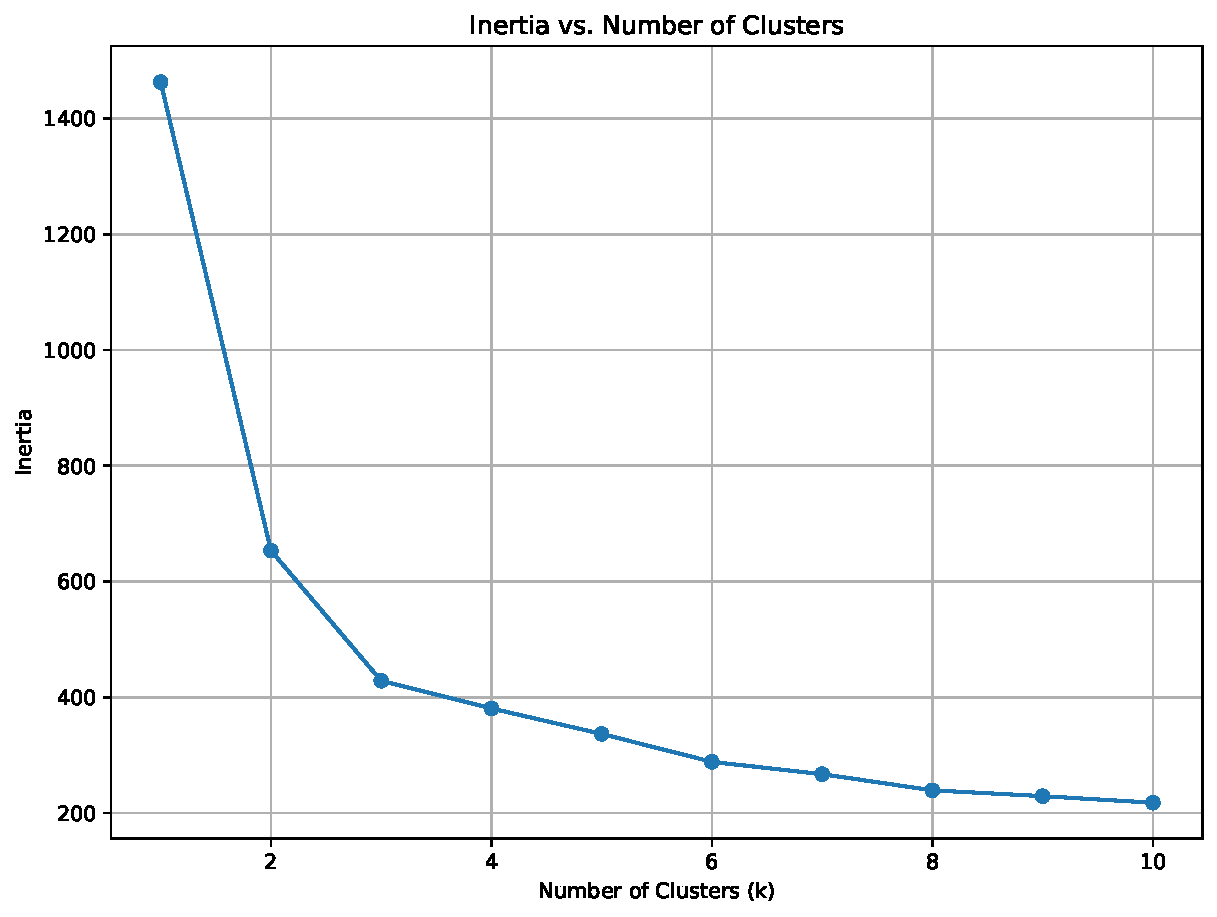
\includegraphics[width=\textwidth]{ola/intertia.pdf}
    \caption{Invertia vs. Number of clusters}
    \label{fig:inertia}
  \end{center}
\end{figure}

\section*{Problem 3: Visualizing the classes}


To visually represent the classes, we initially project all the features onto a 2D plane. 
It becomes evident that the seeds form distinct clusters corresponding to the three species groups. 
However, certain features exhibit less distinct separation than others, such as asymmetry and compactness. 
Notably, the scatter plot depicting the relationship between seed length and width clearly illustrates that seed sizes are readily discernible. 
This is illustrated in Figure~\ref{fig:feature}.

Subsequently, we employ Gaussian random projection to condense the data into a 2D space. 
The outcome is depicted in Figure~\ref{fig:gaussian_random_projection}, where the different seed species remain distinguishable.
 Finally, the UMAP projection is presented in Figure~\ref{fig:umap}, highlighting the distinctiveness of the seed species.

The seeds are indeed distinguishable in the 2D space, particularly through size-related features (area, perimeter, length, width), 
which exhibit a linear relationship. Conversely, other features demonstrate less separability

The ability to distinguish seeds based on size-related features in a 2D space implies that clustering algorithms, 
particularly those sensitive to geometric relationships, can effectively separate seed samples into distinct groups. 
Algorithms like K-means or hierarchical clustering can leverage these separable features to identify natural clusters within the data. 
However, features that are less separable might pose challenges for clustering algorithms, potentially leading to overlapping clusters. 

\begin{figure}[H]
  \begin{center}
    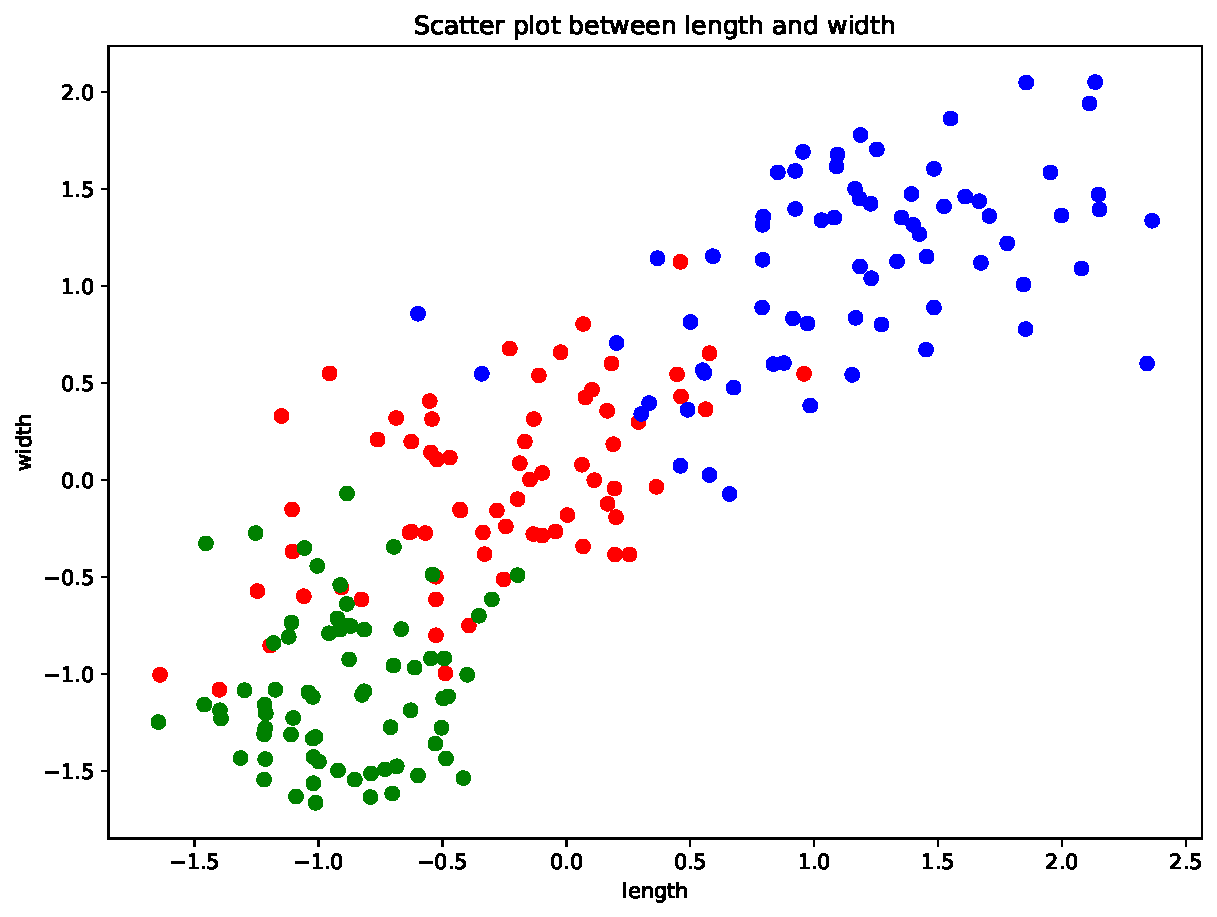
\includegraphics[width=\textwidth]{ola/feature.pdf}
    \caption{Scatter plot between lenght and width}
    \label{fig:feature}
  \end{center}
\end{figure}

\begin{figure}[H]
  \begin{center}
    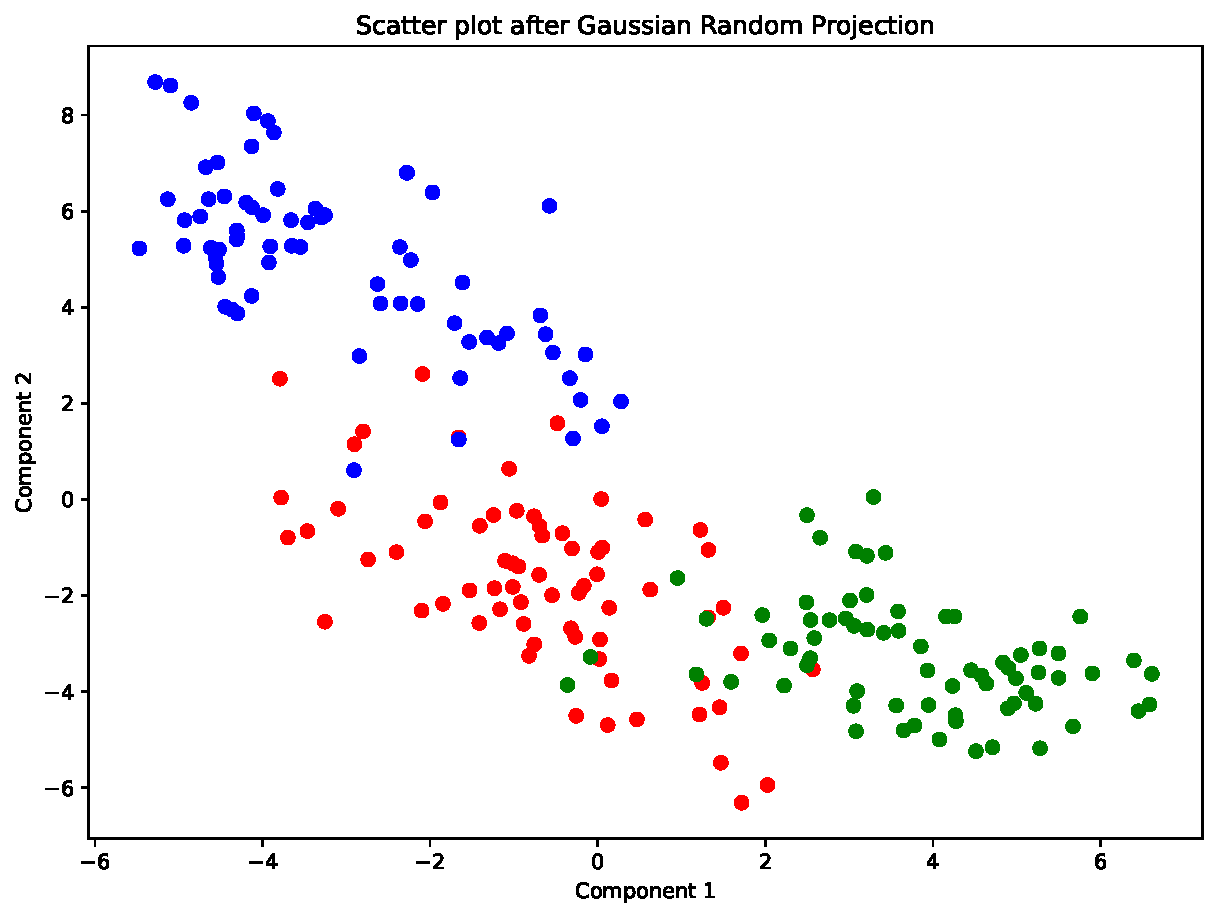
\includegraphics[width=\textwidth]{ola/gaussian_random_projection.pdf}
    \caption{Gaussian random projection}
    \label{fig:gaussian_random_projection}
  \end{center}
\end{figure}

\begin{figure}[H]
  \begin{center}
    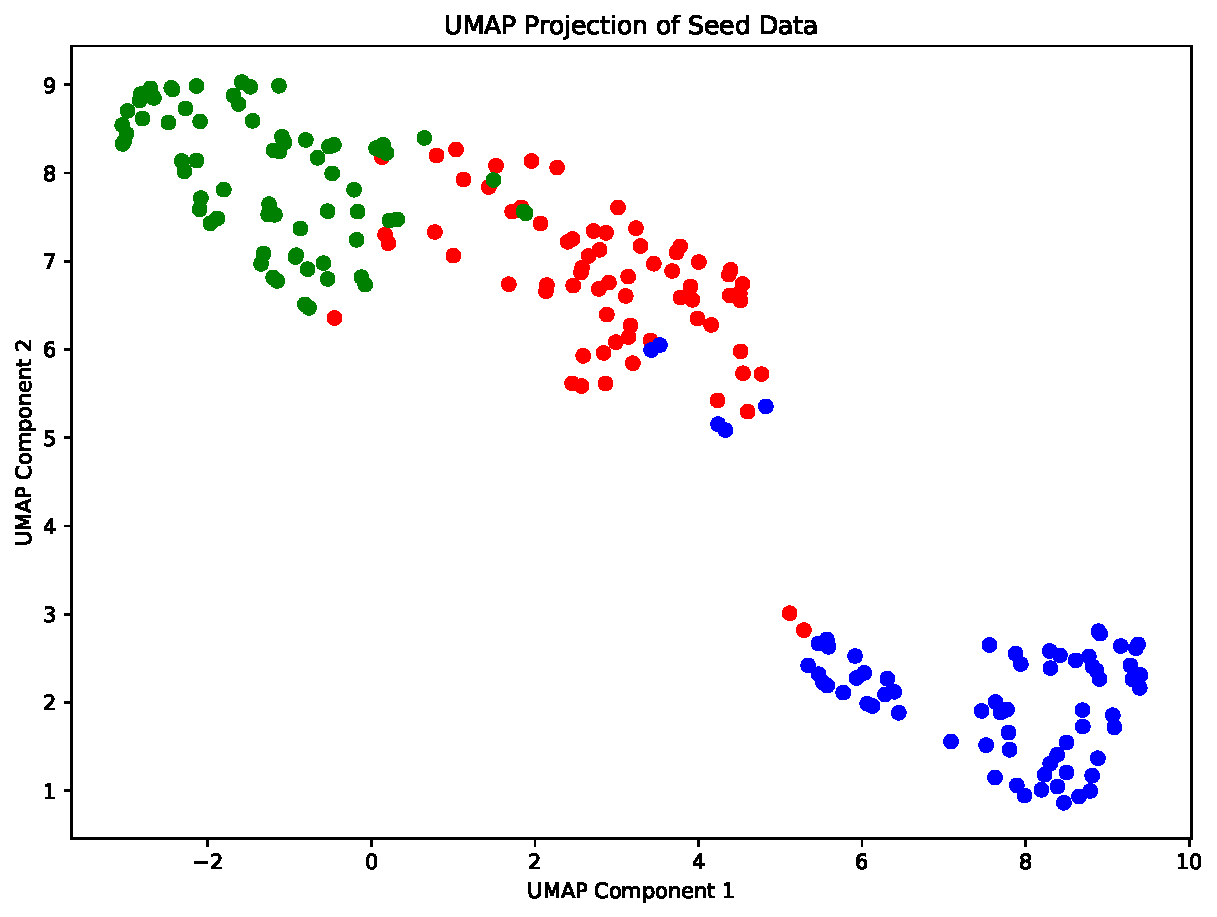
\includegraphics[width=\textwidth]{ola/umap.pdf}
    \caption{UMAP projection of Seeds}
    \label{fig:umap}
  \end{center}
\end{figure}

\section*{Problem 4: Evaluating clustering}
To apply \textit{k}-means clustering to the data, we use the \verb|KMeans| function from \verb|sklearn| with 3 as the number of clusters, and then build the model on the normalized data.

The rand index is obtained by applying the \verb|rand_score| function on the labels of the clustering and the true labels. Its value is 0.90.

Finally we iterate over all the possible permutations in the range $ [0\ldotp\ldotp4] $ to find the best accuracy score. With the permutation $\{0, 1, 2, 3\} \rightarrow \{2, 3, 1, 0\}$, the accuracy is equal to 0.92.

\section*{Problem 5: Agglomerative clustering}
We iterate over the linkage options and calculate the accuracy value after finding the right permutation for each of the linkage options. The best linkage option is the ward method, with an accuracy of 0.93.
The dendrogram is shown in Figure~\ref{fig:dendrogram}

By looking at the 2-dimension projections from Problem 3, some of the points are close neighbors to points that don't belong to the same cluster, and the boundaries between clusters are not clearly defined.
Therefore the "single" linkage option which merge clusters depending on the minimum distance gives a low accuracy value of 0.35.
Other linkage options give roughly the same accuracy (around 0.9).

\begin{figure}[H]
  \begin{center}
    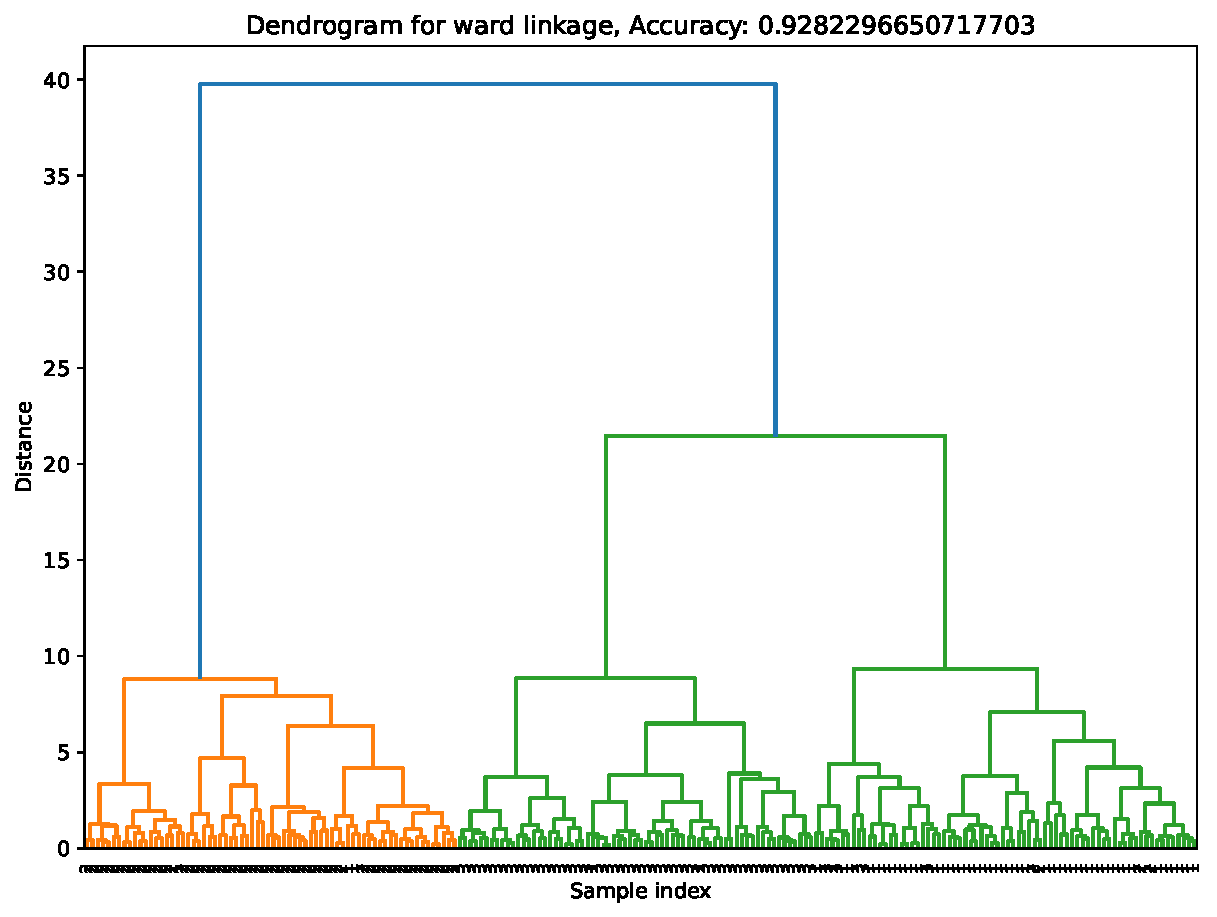
\includegraphics[width=\textwidth]{ola/dendrogram.pdf}
    \caption{Dendrogram}
    \label{fig:dendrogram}
  \end{center}
\end{figure}

\newpage


\printbibliography

\section*{Appendix: Source Code}

\lstset{
  language=Python,
  basicstyle=\ttfamily,
  commentstyle=\color{OliveGreen},
  keywordstyle=\bfseries\color{Magenta},
  stringstyle=\color{YellowOrange},
  numbers=left,
  basicstyle=\footnotesize,
  breaklines=true,
  postbreak=\mbox{\textcolor{red}{$\hookrightarrow$}\space}
}


\lstinputlisting{ola/assignment5.py}

\end{document}
